\documentclass{article}
\usepackage{graphicx}
\usepackage{amsmath}
\usepackage{enumitem}
\usepackage{float}
\usepackage{listings}
\usepackage{xcolor}
\usepackage{caption}
\usepackage[a4paper, margin=1in]{geometry}

% Custom information
\newcommand{\className}{Course: Automatic Control Systems – ASEN 5114-001 – Spring 2025}
\newcommand{\professorName}{Professor: Dale Lawrence}
\newcommand{\taName}{Teaching Assistant: Anantha Dhruva}
\title{Midterm \\ \className \\ \professorName \\ \taName}
\author{Steve Gillet}
\date{\today}

\lstdefinestyle{matlabstyle}{
    language=Matlab,              % Specify the language
    basicstyle=\ttfamily\footnotesize\color{black}, % Code font
    keywordstyle=\color{blue}\bfseries, % Keywords in blue
    stringstyle=\color{orange},    % Strings in orange
    commentstyle=\color{magenta}, % Comments in magenta
    numbers=left,                 % Line numbers on the left
    numberstyle=\tiny\color{black},% Line number style
    stepnumber=1,                 % Line number increment
    breaklines=true,              % Line breaking
    frame=single,                 % Border around code
    backgroundcolor=\color{white},
    tabsize=4,                    % Tab size
    showstringspaces=false,       % Don't show spaces in strings
}

\renewcommand{\thesection}{\arabic{section})}
\renewcommand{\thesubsection}{\arabic{section}.\arabic{subsection}}

\begin{document}

\maketitle

\textit{The following take-home midterm exam must be completed individually by each student. Students may use their notes, or the textbook. Any other resources used must be cited. Students are NOT allowed to communicate with any other person, except the instructor. Show your work and justify your answers for full credit. This exam is due at 11:59 PM on Monday, February 24 on Canvas. Students registered for ASEN 5114 do problems 2,3,4,5. Students registered for ASEN 4114 do problems 1,3,4,5.}

\setcounter{section}{1}
\section{}

\textit{[40 pts] Find a direct state space model for the mechanical system at right, with an input force $f_a(t)$ oriented positive downward on $M_2$ and output $\omega(t)$. Neglect gravity and assume all positions are measured from the nominal position where the springs are at their rest length. The pinion gear with radius $R_2$ meshes with a rack gear on the side of $M_2$ without slipping. Model the sliding friction $B$ with a linear damper. Note the rotating shaft has torsional stiffness $K_2$. Order the states in this model according to the element indexes, starting with inertial elements. Do not use the symbol "x" for state variables, since these are already used for displacements in the figure. $\theta$ and $\omega$ are inertially referenced.}

\begin{figure}[H]
    \centering
    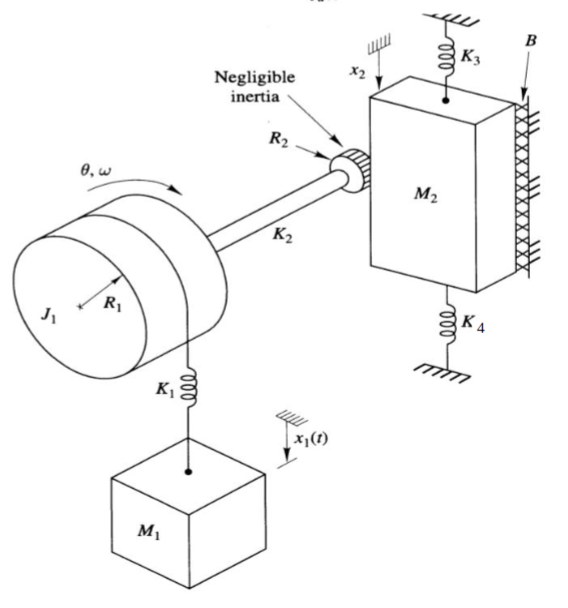
\includegraphics[width=0.5\textwidth]{q2fig.png}
\end{figure}

\subsection*{1) Identify}
\begin{itemize}
    \item Input: \( u = f \)
    \item Output: \( y = \omega \)
    \item States:
    \begin{itemize}
        \item Mass \( M_1 \): \( w_1 = v_{M_1} \)
        \item Spring \( K_1 \): \( w_2 = f_{K_1} \)
        \item Mass \( M_2 \): \( w_3 = v_{M_2} \)
        \item Spring \( K_3 \): \( w_4 = f_{K_3} \)
        \item Spring \( K_4 \): \( w_5 = f_{K_4} \)
        \item Mass \( J_1 \): \( w_6 = \omega = y \)
        \item Mass \( M_2 \): \( w_7 = x_2 \)
        \item Mass \( J_1 \): \( w_8 = \Theta \)
    \end{itemize}
\end{itemize}

\subsection*{2) Complementary State Variables}
\[
w_1^* = f_{M_1}, \quad w_2^* = v_{K_1}, \quad w_3^* = f_{M_2}, \quad w_4^* = v_{K_3}, \quad w_5^* = v_{K_4}, \quad w_6^* = \tau_{J_1}
\]

\subsection*{3) Topology Equations}
\begin{align*}
w_1^* &= f_{M_1} = -f_{K_1} = -w_2 \\
w_2^* &= v_{K_1} = v_{M_1} - \omega = w_1 - w_6 \\
w_3^* &= f_{M_2} = f - B v_{M_2} + f_{K_4} - f_{K_3} - K_2 \left( \Theta - \frac{x_2}{R_2} \right) \\
      &= f - B w_3 + w_5 - w_{4} - K_2 \left( w_8 - \frac{w_2}{R_2} \right) \\
w_4^* &= v_{K_3} = v_{M_2} = w_3 \\
w_5^* &= v_{K_4} = -v_{M_2} = -w_3 \\
w_6^* &= \tau_{J_1} = f_{K_1} - K_2 \left( \theta - \frac{x_2}{R_2} \right) = w_2 - K_2 \left( w_8 - \frac{w_7}{R_2} \right)
\end{align*}

\subsection*{4) Energy Storage Element Equations}
\begin{align*}
w_1^* &= f_{M_1} = M_1 \dot{v}_{M_1} = M_1 \dot{w}_1 \implies \dot{w}_1 = - \frac{1}{M_1} w_2 \\
w_2^* &= v_{K_1} = \frac{1}{K_1} \dot{f}_{K_1} = \frac{1}{K_1} \dot{w}_2 \implies \dot{w_2} = K_1 (w_1 - w_6) \\
w_3^* &= f_{M_2} = M_2 \dot{v}_{M_2} = M_2 \dot{w}_3 \implies \dot{w}_3 = \frac{1}{M_2} (f - B w_3 + w_5 - w_4 - K_2 (w_8 - \frac{w_7}{R_2})) \\
w_4^* &= v_{K_3} = \frac{1}{K_3} \dot{f}_{K_3} = \frac{1}{K_3} \dot{w}_4 \implies \dot{w}_4 = K_3 w_3 \\
w_5^* &= v_{K_4} = \frac{1}{K_4} \dot{f}_{K_4} = \frac{1}{K_4} \dot{w_5} \implies \dot{w_5} = -K_4 w_3 \\
w_6^* &= \tau_{J_1} = J_1 \dot{\omega} = J_1 \dot{w}_6 \implies \dot{w}_6 = \frac{1}{J_1} w_2 - \frac{K_2}{J_1} w_8 + \frac{K_2}{J_1 R_2} w_7
\end{align*}
Note: \( \dot{w}_7 = w_3 \), \( \dot{w}_8 = w_6 \)

\subsection*{5) Matrix Form}
State vector: \( \mathbf{w} = [w_1, w_2, w_3, w_4, w_5, w_6, w_7, w_8]^T \)

State-space equations:
\[
\mathbf{\dot{w}} = A \mathbf{w} + B u, \quad y = C \mathbf{w} + D u
\]
Where:
\[
A = \begin{bmatrix}
0 & -\frac{1}{M_1} & 0 & 0 & 0 & 0 & 0 & 0 \\
K_1 & 0 & 0 & 0 & 0 & -K_1 & 0 & 0 \\
0 & 0 & -\frac{1}{M_2} & -\frac{1}{M_2} & \frac{1}{M_2} & 0 & \frac{K_2}{M_2} & -\frac{K_2}{M_2} \\
0 & 0 & K_3 & 0 & 0 & 0 & 0 & 0 \\
0 & 0 & 0 & -K_4 & 0 & 0 & 0 & 0 \\
0 & \frac{1}{J_1} & 0 & 0 & 0 & 0 & \frac{K_2}{J_1 R_1} & -\frac{K_2}{J_1} \\
0 & 0 & 1 & 0 & 0 & 0 & 0 & 0 \\
0 & 0 & 0 & 0 & 0 & 1 & 0 & 0
\end{bmatrix}
\]
\[
B = \begin{bmatrix} 0 \\ 0 \\ \frac{1}{M_2} \\ 0 \\ 0 \\ 0 \\ 0 \\ 0 \end{bmatrix}, \quad
C = \begin{bmatrix} 0 & 0 & 0 & 0 & 0 & 1 & 0 & 0 \end{bmatrix}, \quad
D = \begin{bmatrix} 0 \end{bmatrix}
\]

\end{document}